
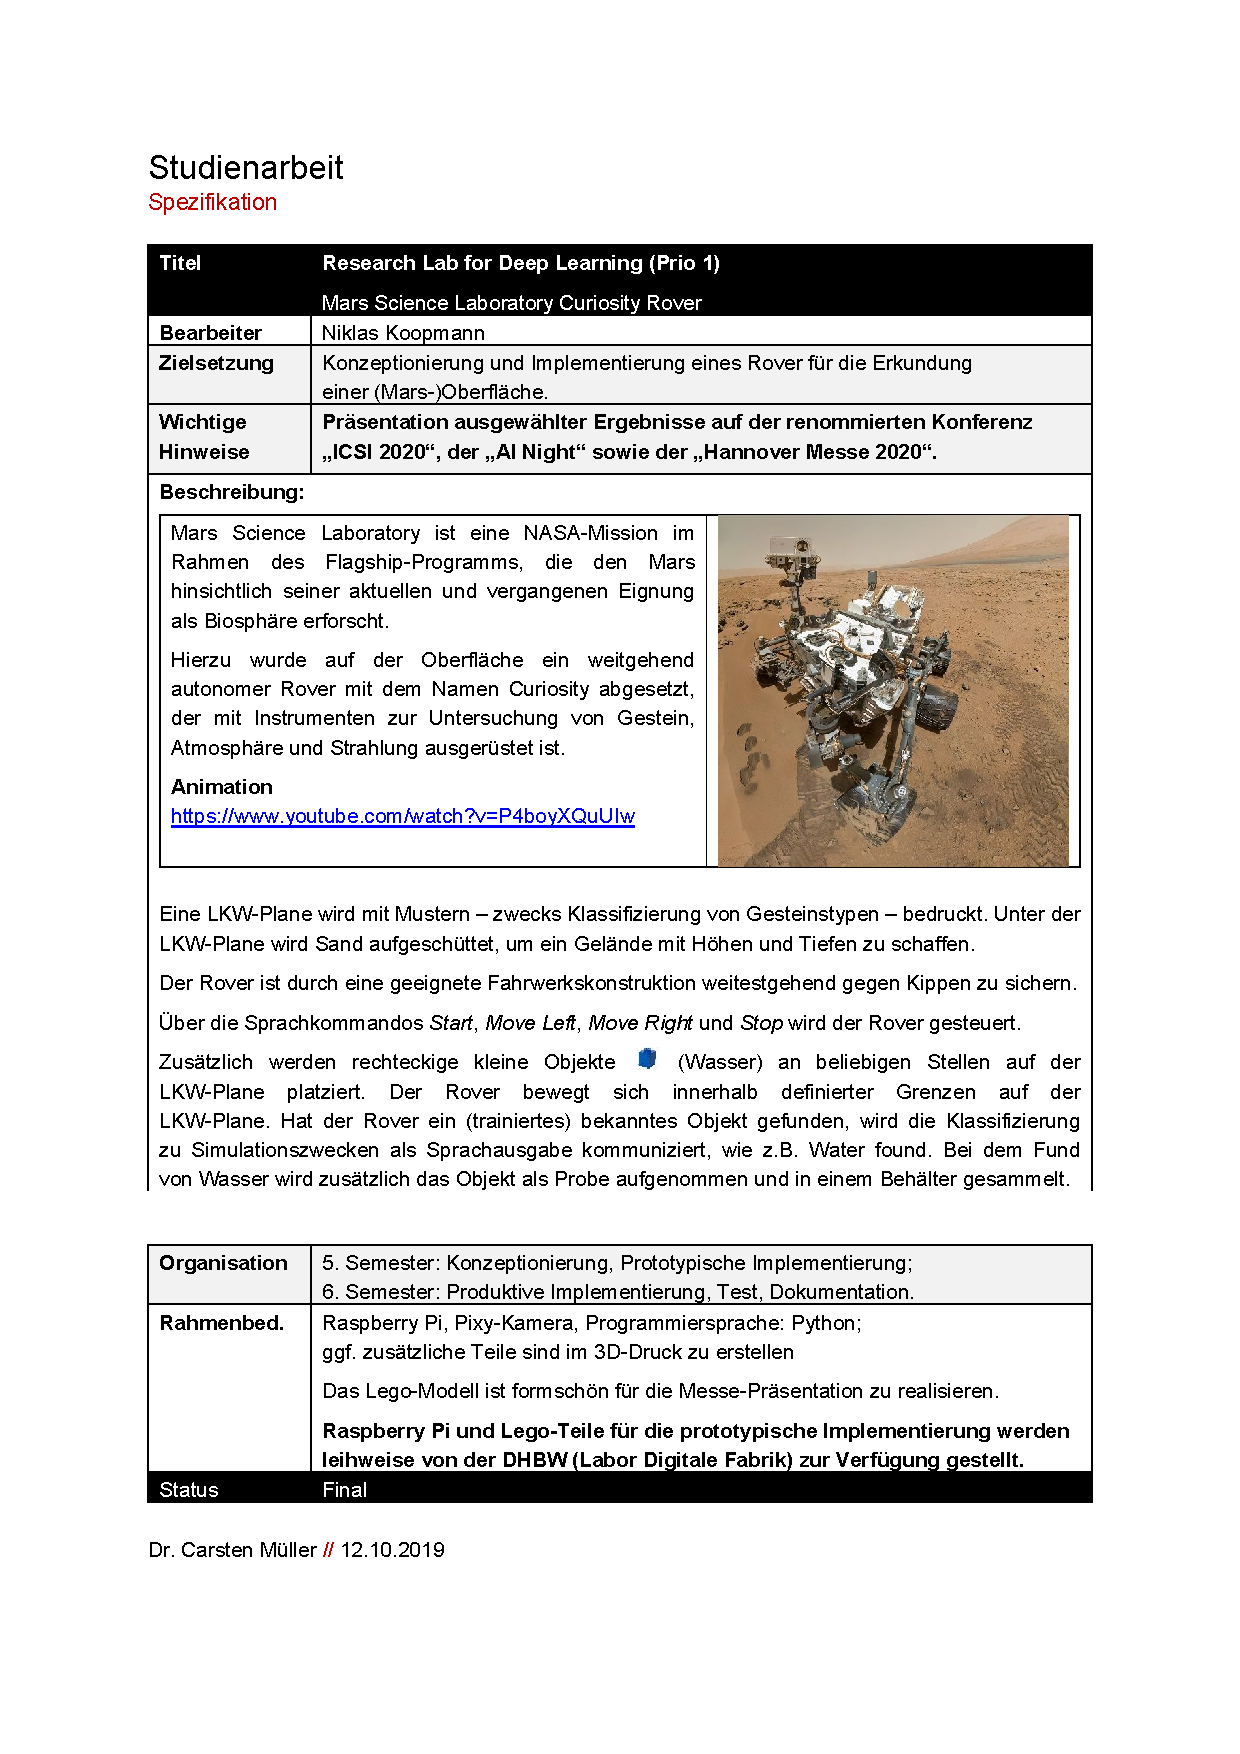
\includepdf[scale=0.8, pages=1, offset=0 -1cm, pagecommand={\chapter{Spezifikation} \label{chp:spezifikation}}]{content/spec.pdf}
\includepdf[scale=0.8, pages=2-, offset=0 -1cm, pagecommand={}]{content/spec.pdf}

\section{Motivation}
\label{sec:motivation}

Am 6. August 2012 landete der Rover \textit{Curiosity} als Teil der Mission \textit{Mars Science Laboratory} der US-amerikanischen Raumfahrtbehörde \acf{nasa} \cite{vasavada2014}.
Seither hat er rund $21{,}93$ Kilometer zurückgelegt (Stand: Sol 2695) \cite{nasa2020}.
% TODO Mehrwert für die Wissenschaft

...

Dieses Projekt wird im Rahmen des Research Lab for Deep Learning der Dualen Hochschule Baden-Württemberg (\acsu{dhbw}) zeitgleich mit der Erforschung schwarmbasierter Logistikabläufe durchgeführt.
Langfristig soll es unter anderem zum Zwecke einer schwarmbasierten Erkundung marsähnlicher Landschaften weiterentwickelt werden können.

\section{Aufgabenstellung}
\label{sec:aufgabe}

Ziel dieser Arbeit ist die \glqq Konzeptionierung und Implementierung eines Rover für die Erkundung einer (Mars-)Oberfläche\grqq\ \cite{mueller2019}.

% TODO REMOVE LITERATURE TESTS
Literatur-Test:
\cite{yamanoor2017}
\cite{horan2013}
\cite{molloy2016}
\cite{donat2018}
\cite{halfacree2019}
\cite{cole2013}
\cite{mcmanus2017}
\cite{cox2014}
\cite{pajankar2015}
\cite{pagnutti2017}